\subsection{Súčasný stav na trhu}
Ak hovoríme o heslách, priame (explicitné) používanie nižšie uvedených aplikácií pri dennom používaní je minimálne. A to vďaka automatickému vypĺňaniu hesla. Používateľ vstúpi na webovú stránku alebo do aplikácie. Pred vstupom sa musí prihlásiť do svojho účtu. Tam mu password manager výzvou ponúkne automatické vyplnenie (angl. výraz ,,autofill'') prihlasovacieho mena a hesla. Toto poskytuje vysokú úroveň komfortu. Používateľ nielen že nemusí vypisovať svoje prihlasovacie údaje manuálne, ale aj ich bezpečnosť porástla na vyššiu úroveň. Vďaka password manageru.
\par Podobne to funguje pri registrácii nového konta. Niektoré password manager aplikácie ponúknu náhodne vygenerované silné heslo (iCloud Keychain, \cite{10}). Používateľ sa môže rozhodnúť ho prijať. V takom prípade sa heslo pre vytvorený účet uloží do password manageru a ten ho pri každom ďalšom prihlásení vyplní. 
\subsubsection{LastPass} 
LastPass patrí medzi jeden z najpopulárnejších, čo sa týka počtu používateľov \cite{11}. Všetky heslá a ostatný obsah sú uzamknuté pod jedným master heslom. LastPass ale povoľuje aj vstup do jeho aplikácie pomocou biometrickej autentifikácie, ktorú väčšina smartfónov podporuje. Používateľ tak nemusí každý raz písať dlhé master heslo. Jediné, čo stačí, je priložiť prst, či pozrieť sa na smartfón (sken tváre). 
\par LastPass je client-server aplikácia. To znamená, že niektoré operácie a procesy prebiehajú na strane kienta, teda priamo v danom zariadení, ktoré používateľ drží a niektoré prebiehajú na strane LastPass serverov. Samotné šifrovanie, aj dešifrovanie prebieha na strane zariadenia \cite{12}. LastPass vytvorí kľúč z master hesla pomocou šifry AES (Advanced Encryption Standard) s hašovaním PBKDF2 (Key Derivation Function), SHA (Secure Hash Algorithm) s pridaným saltom \cite{13}. Týmto algoritmom sa bližšie venujeme v X.X (TODO číslo sekcie kde budem vysvetľovať AES princíp a hašovanie).
\par Dáta sú synchronizované pomocou serverov, čo umožňuje zálohovanie a synchronizáciu medzi zariadeniami. Dátový prenos po sieti je chránený pomocou TLS/SSL (\cite{14} sa bližšie venuje tomuto protokolu). LastPass v bezpečnosti pokračuje v možnosti dvojfaktorovej autorizácie a overovania na základe lokácie: kedykoľvek sa užívateľ prihlasuje do aplikácie z inej lokality, je vyzvaný prostredníctvom emailu s linkom, ktorý po otvorení overí používateľa ako verifikovaného. LastPass má mnoho možností, ako napríklad zdieľanie hesiel s iným LastPass účtom, generovanie hesiel s používateľom zvolenou dĺžkou a podmienkami, hodnotenie sily hesiel (systém usúdi, či je heslo dostatočne bezpečné), či import hesiel pomocou CSV súboru alebo iného password manageru.
\newline
\begin{figure}[ht]
  \centering
  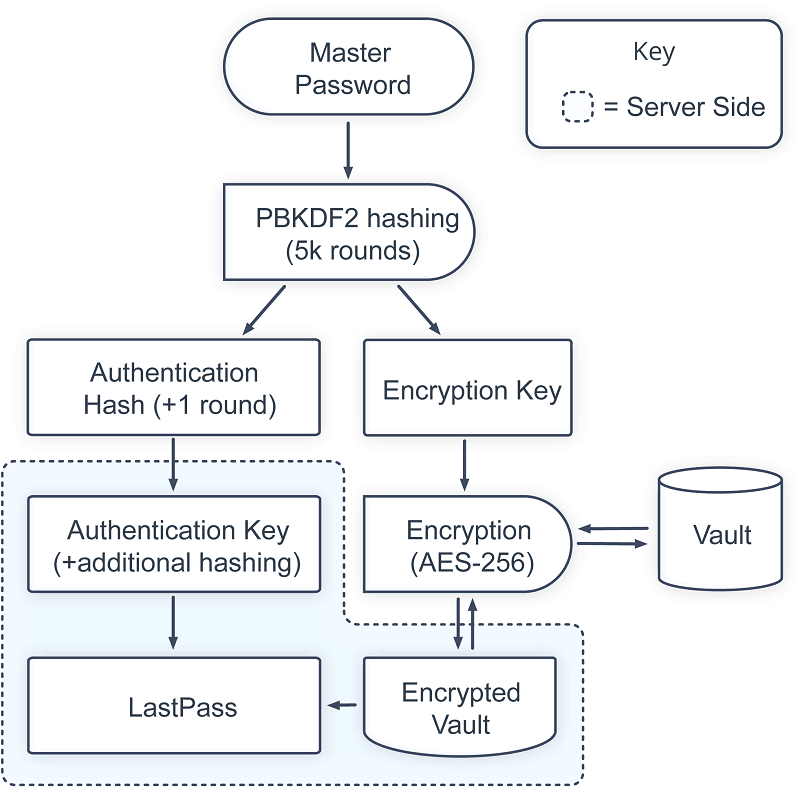
\includegraphics[width=8cm]{img/lastpass.png}
  \caption{Schéma šifrovania aplikácie LastPass.}
\end{figure}

\subsubsection{Dashlane}
Tento password manager je tiež vysoko využívaný \cite{15}. Jedna z jeho jedinečných funkcionalít je automatická zmena hesla \cite{16}. Používateľ si môže vybrať v zozname svojich hesiel, ktoré by sa mali automaticky meniť. Dashlane tak bude pravidelne generovať nové, komplexné heslá pre vybrané položky. Keďže medzi rôznymi webovými stránkami nie je jednotná architektúra a dizajn, nie všetky položky účtov vie Dashlane meniť automaticky. V takom prípade si užívateľ vie meniť heslo pre danú položku iba manuálne, v konkrétnej aplikácii alebo webovej stránke pre službu, ku ktorej prislúcha daný účet v Dashlane.
\par Tak ako LastPass, aj tento password manager dominuje silnou bezpečnosťou. Podporuje dvojfaktorovú autentifikáciu (dodatočné overenie po prvotnom prihlásení, viac v \cite{17}), šifru AES a synchronizáciu medzi zariadeniami. Mnohé z funkcionalít a možností má spoločné s aplikáciou LastPass. Nebudeme ich opäť spomínať, nakoľko cieľom tejto kapitoly je iba ukázať už existujúce vymoženosti rôznych password managerov.

\subsubsection{iCloud Keychain}
\par Za spomenutie určite stojí vstavaný password manager od spoločnosti Apple. Obsahuje určité funkcionality password managera, ktoré sú základnou súčasťou každého iOS, iPadOS, či MacOS zariadenia. Každý používateľ nejakého Apple zariadenia je identifikovaný pomocou AppleID konta. K nemu má pridelené cloud úložisko, kde sa mu všetky dáta zálohujú a synchronizujú so všetkými Apple zariadeniami.
\par Okrem fotiek, poznámok, kontaktov a iných dát tam sú uložené aj heslá z Keychainu. Keychain si pamätá nielen heslá, ale aj certifikáty, dôležité pri rôznych verifikáciach v rámci systému. Taktiež si pamätá kľúče. Sú verejné, ale aj súkromné, systém ich používa napríklad pri používaní iMessage (četovacia aplikácia). Sú šifrované pomocou šifry RSA a dĺžka kľúča je niekedy až 2048 bitov. \\

\par Z ostatných managerov ukážeme zopár ďalších funkcionalít, ktoré neboli spomenuté, respektíve ich LastPass, Dashlane, či Keychain neposkytujú.
\par 1Password ponúka takzvaný ,,Emergancy kit''. Po vytvorení 1Password účtu je používateľovi poskytnutý dokument. Následne je vyzvaný, aby si ho vytlačil, prípadne uložil na pamäťové médium. Dokument obsahuje prihlasovacie údaje a master heslo. Taktiež obsahuje QR kód, ktorý automaticky vyplní tieto dáta pri núdzovom prihlasovaní. \\

\begin{figure}[ht]
  \centering
  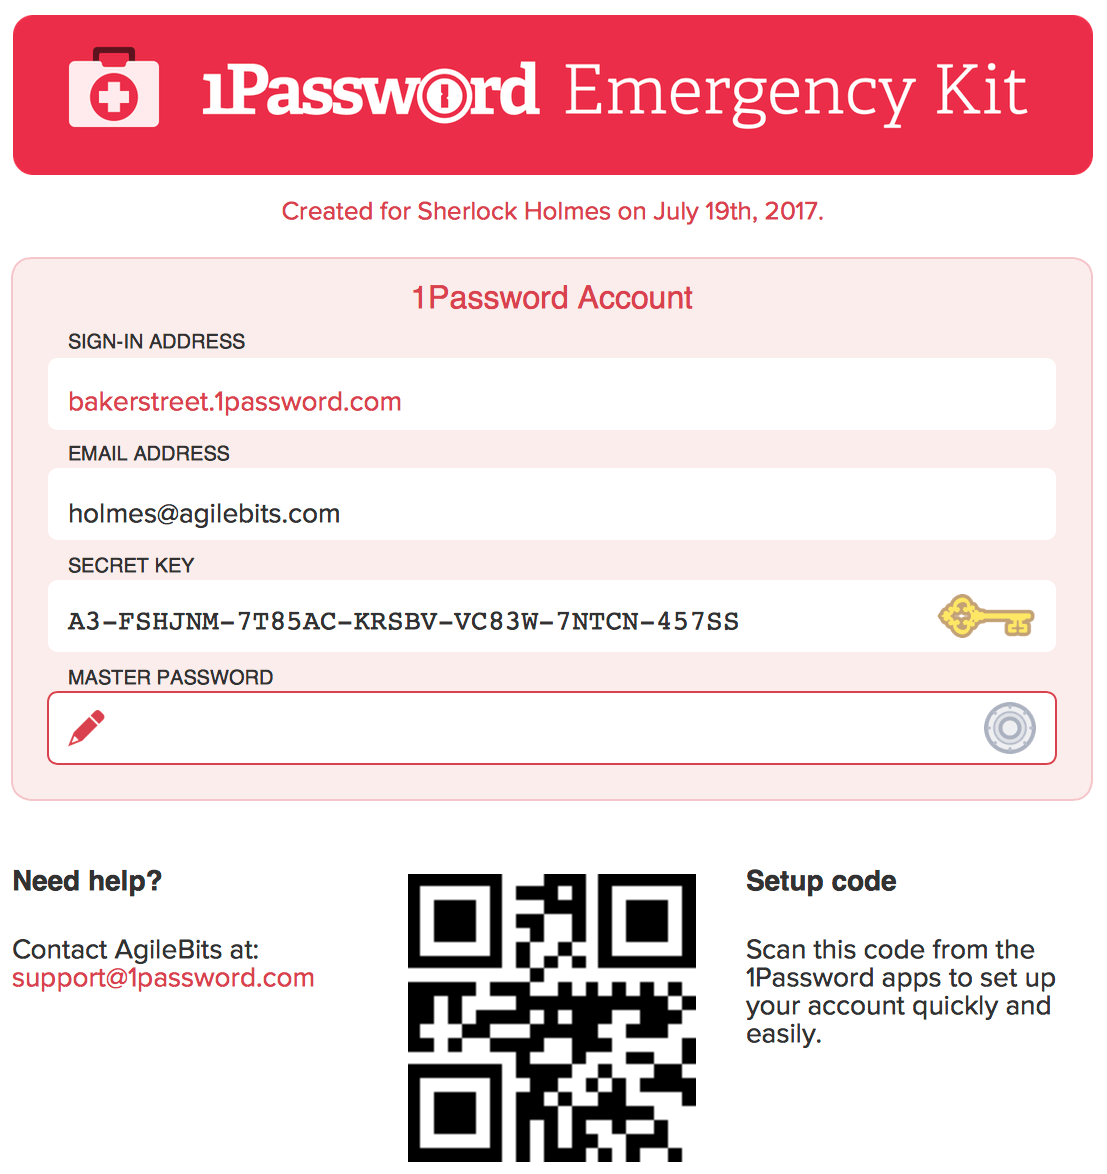
\includegraphics[width=8cm]{img/1pass.png}
  \caption{Emergency kit od 1Password - ukážka pdf súboru, ktorý používateľ obdrží.}
\end{figure}

\par Password manager Remembear ponúka jednoduchú aktiváciu aplikácie na novom zariadení prostredníctvom QR kódu. Za spomenutie stojí aj menej známy správca, konkrétne Myki. \par Myki ako jeden z mála nepoužíva svoje servery na zálohovanie a ukladanie hesiel. Namiesto toho využíva server iba ako sprostredkovateľa \cite{18} spojenia keď nastáva synchronizácia medzi zariadeniami. Teda, používať Myki na viacerých zariadeniach je akousi formou ,,zálohy''.
\par Vyššie spomenuté aplikácie fungujú na rôznych platformách: verzia pre smartfóny (iOS, Android), počítače (Windows, MacOS, Linux), inteligentné hodinky a podobne.